%\chapter{Guerra de Sucesión}

La guerra enfrentaba a Felipe de Anjou, apoyado por Francia y nombrado
heredero por el difunto rey español, con el archiduque Carlos de
Austria, apoyado por Inglaterra, ya que esta última temía el poderío
que alcanzarían los Borbones en el continente en caso de unirse las
dos coronas, española y francesa. Para recuperar
Gibraltar\index{Gibraltar|textbf} ---tomado
por las fuerzas anglo-holandesas--- y desbloquear el acceso al
Mediterráneo, franceses y españoles aprestaron una gran armada
(cfr. \cite{qui01,garciarivas}).\index{armada} La escuadra francesa había salido de
Tolón y en Málaga se habían unido a ella algunas galeras españolas
mandadas por el conde de Fuencalada. Frente a Vélez-Málaga se produjo
el 24 de agosto de 1704 la batalla naval más importante del
conflicto. En dicho combate se enfrentaron 96 naves de guerra
franco-españolas (51 navíos de línea, seis fragatas, ocho brulotes y
doce galeras, que sumaban un total de 3577 cañones y 24277 hombres) y
la flota anglo-holandesa, mandada por el almirante Rooke y compuesta
por 53 navíos de línea, seis fragatas, pataches y brulotes con un
total de 3614 cañones y 22543 hombres, dando como resultado al final
de la contienda 1500 y 2719 bajas, respectivamente.

Blas de Lezo participó en aquella batalla batiéndose de manera
ejemplar,\index{Blas de Lezo} hasta que, poco después de comenzar el
combate, una bala de cañón le destrozó la pierna izquierda
(cfr. \cite{qui01}), teniéndosela que amputar, sin anestesia, por
debajo de la rodilla. Debido al valor demostrado tanto en aquel trance
como en el propio combate, fue ascendido en 1704 a alférez de bajel de
alto bordo por Luis XIV, al que el comandante francés había notificado
la bizarría de Lezo. Felipe V le otorgó también una merced de hábito,
que conllevaba una serie de privilegios similares a los de la baja
aristocracia.

\begin{figure}[!hbp]
\centering
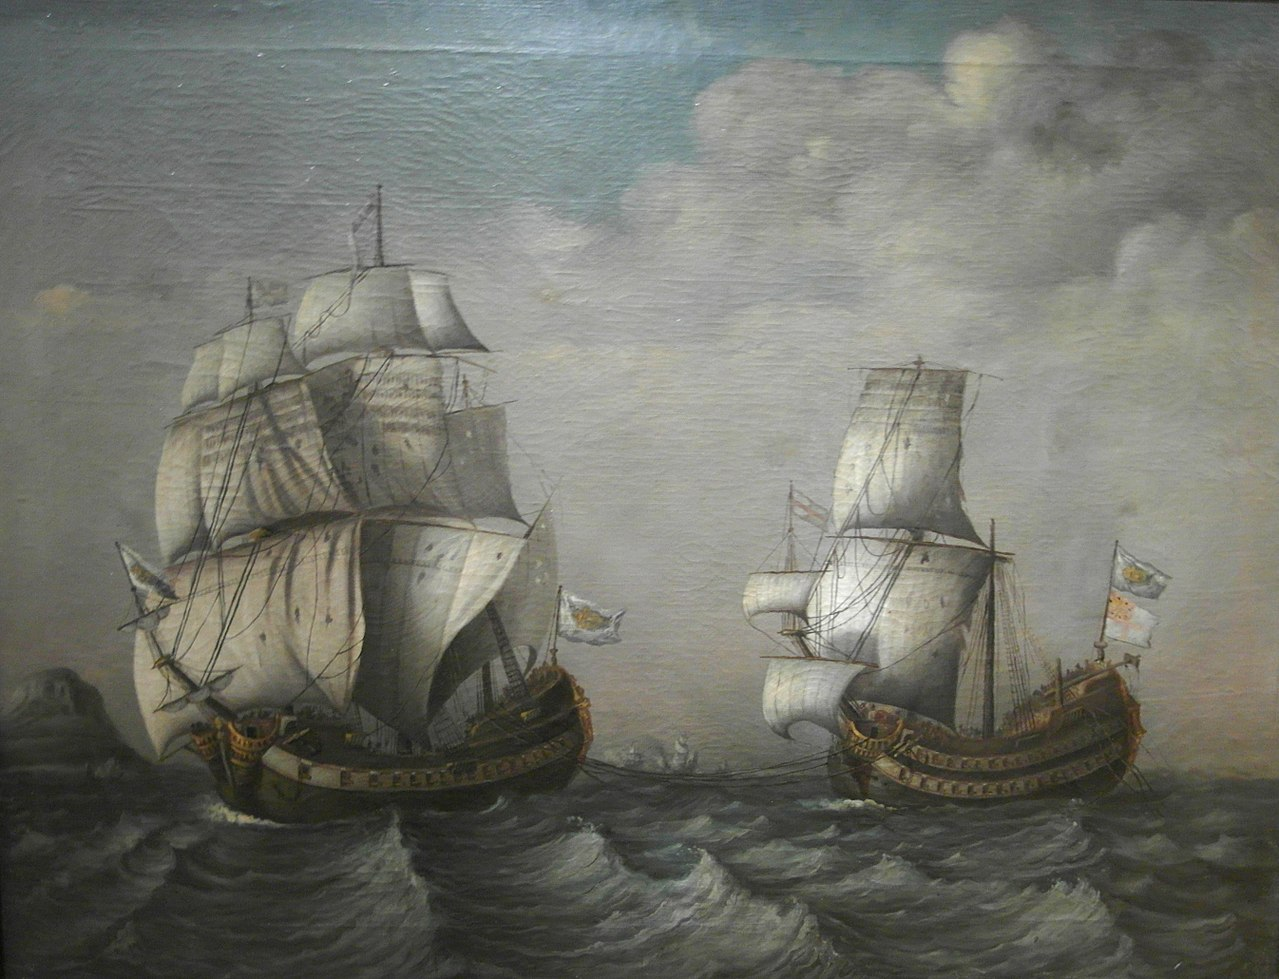
\includegraphics[width=.35\textwidth]{jpg_LaFragataDeBlasDeLezoRemolcandoAlStanhopeHaci1710.jpg}
\caption{\label{fig:fragata} La fragata de D. Blas de Lezo remolcando
al buque británico \textit{Stanhope}.}
\end{figure}

Se le ofreció ser asistente de cámara de la Corte de Felipe V. Rechazó
este cargo y, una vez recuperado de la pérdida de la pierna, siguió su
servicio a bordo de diferentes buques, tomando parte en las
operaciones que tuvieron lugar para socorrer las plazas de Peñíscola y
Palermo; en el ataque al navío inglés Resolution de setenta cañones en
la costa genovesa, que terminó con la quema de este; así como en el
apresamiento posterior de dos navíos enemigos en el Mediterráneo
occidental, que fueron conducidos a Pasajes y Bayona, todo ello en
1705. El mando de las presas se otorgaba como premio a los oficiales
que se habían distinguido en el servicio, como debió de hacer Lezo en
los combates de ese año.

Evidentemente necesitó una larga recuperación y rechazó estar en la
Corte, pues ambicionaba conocer las artes marineras y convertirse en
un gran comandante.

Pero enseguida es requerido por sus superiores y en 1706 se le ordenó
abastecer a los sitiadores de Barcelona al mando de una pequeña
flotilla, parte de la armada \index{armada} que con este fin mandaba
un almirante francés. Realizó brillantemente su cometido, escapando
una y otra vez de las naves enemigas y facilitando el
aprovisionamiento del ejército del mariscal de Tessé. Para ello deja
flotando y ardiendo paja húmeda con el fin de crear una densa nube de
humo que ocultase los navíos españoles, pero además carga ``sus
cañones con unos casquetes de armazón delgada con material incendiario
dentro, que, al ser disparados, prenden fuego a los buques
británicos'' (cfr. \cite{garciarivas}). Los británicos se ven
impotentes ante tal despliegue de ingenio.

Posteriormente se le destacó a la fortaleza de Santa Catalina de
Tolón, donde participó en la defensa de la base naval francesa de la
acometida de la flota del príncipe Eugenio de Saboya. En esta acción y
tras el impacto de un cañonazo en la fortificación, una esquirla le
reventó el ojo izquierdo.
